Een condensator\index{Condensator}\index{Capacitor} bestaat uit twee platen van een geleidend materiaal dat bescheiden wordt door een isolator, een zogenaamd di\"electricum. Als er een spanning gezet wordt op een circuit met een condensator erin dan zullen de elektronen naar de plus pool willen bewegen, daardoor worden er elektronen aan de plaat die aan de plus pool hangt onttrokken, deze zal dan positief geladen worden. Bij de min-pool gebeurt precies het omgekeerde en de plaat aan de min-pool wordt nu negatief geladen. Koppelen de we batterij los, dan houden we een geladen condensator over, met een spanning die gelijk is aan de spanning van de batterij.

De hoeveelheid lading die we op een condensator kunnen opslaan is beperkt, dus hij is dan ook zo weer leeg gelopen. Een condensator werkt dus als een mini-batterij.

In de elektronica wordt een condensator weergegeven met het symbool dat je ziet weergegeven in \ref{symbool:condensator}

\begin{figure}[h]
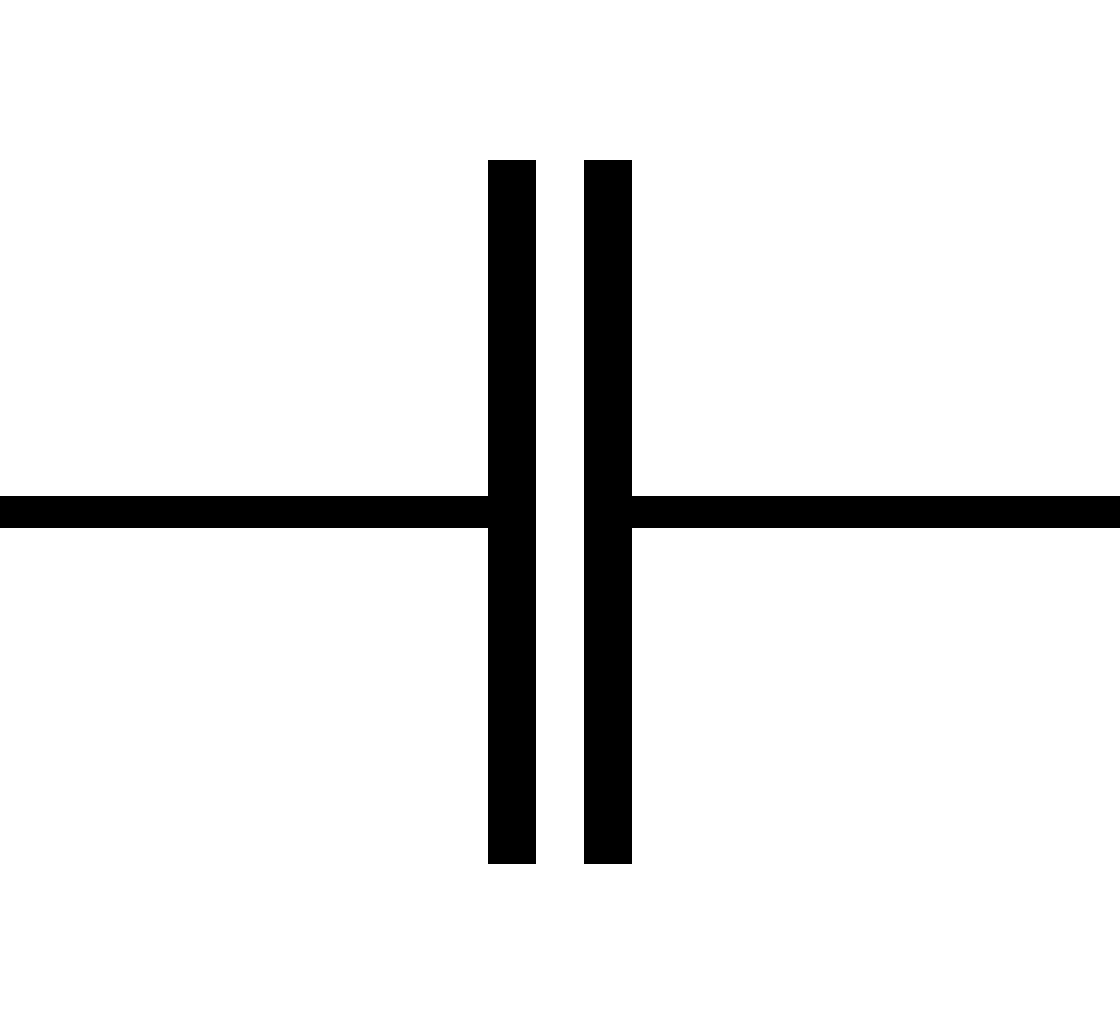
\includegraphics[width=5cm]{condensator}
\centering
\caption{Symbool van een condensator}
\label{symbool:condensator}
\end{figure}

